\documentclass[a4paper, 11pt]{ctexart}

%%%%% 导入包 %%%%%%
\usepackage{graphicx}
\usepackage[unicode]{hyperref}
\usepackage{xcolor}
\usepackage{cite}
\usepackage{indentfirst}
\usepackage{amsmath}
\usepackage{longtable}
\usepackage{listings} % 导入 listings 包
\graphicspath{{Figures/}}%文章所用图片在当前目录下的 Figures目录

%%%%% 设置字号 %%%%%%
\newcommand{\chuhao}{\fontsize{42pt}{\baselineskip}\selectfont}
\newcommand{\xiaochuhao}{\fontsize{36pt}{\baselineskip}\selectfont}
\newcommand{\yihao}{\fontsize{28pt}{\baselineskip}\selectfont}
\newcommand{\erhao}{\fontsize{21pt}{\baselineskip}\selectfont}
\newcommand{\xiaoerhao}{\fontsize{18pt}{\baselineskip}\selectfont}
\newcommand{\sanhao}{\fontsize{15.75pt}{\baselineskip}\selectfont}
\newcommand{\sihao}{\fontsize{14pt}{\baselineskip}\selectfont}
\newcommand{\xiaosihao}{\fontsize{12pt}{\baselineskip}\selectfont}
\newcommand{\wuhao}{\fontsize{10.5pt}{\baselineskip}\selectfont}
\newcommand{\xiaowuhao}{\fontsize{9pt}{\baselineskip}\selectfont}
\newcommand{\liuhao}{\fontsize{7.875pt}{\baselineskip}\selectfont}
\newcommand{\qihao}{\fontsize{5.25pt}{\baselineskip}\selectfont}

%%%% 设置 section 属性 %%%%
\makeatletter
\renewcommand\section{\@startsection{section}{1}{\z@}%
{-1.5ex \@plus -.5ex \@minus -.2ex}%
{.5ex \@plus .1ex}%
{\normalfont\sihao\CJKfamily{hei}}}
\makeatother

%%%% 设置 subsection 属性 %%%%
\makeatletter
\renewcommand\subsection{\@startsection{subsection}{1}{\z@}%
{-1.25ex \@plus -.5ex \@minus -.2ex}%
{.4ex \@plus .1ex}%
{\normalfont\xiaosihao\CJKfamily{hei}}}
\makeatother

%%%% 设置 subsubsection 属性 %%%%
\makeatletter
\renewcommand\subsubsection{\@startsection{subsubsection}{1}{\z@}%
{-1ex \@plus -.5ex \@minus -.2ex}%
{.3ex \@plus .1ex}%
{\normalfont\xiaosihao\CJKfamily{hei}}}
\makeatother

%%%% 段落首行缩进两个字 %%%%
\makeatletter
\let\@afterindentfalse\@afterindenttrue
\@afterindenttrue
\makeatother
\setlength{\parindent}{2em}  %中文缩进两个汉字位

%%%% 下面的命令重定义页面边距,使其符合中文刊物习惯 %%%%
\addtolength{\topmargin}{-54pt}
\setlength{\oddsidemargin}{0.63cm}  % 3.17cm - 1 inch
\setlength{\evensidemargin}{\oddsidemargin}
\setlength{\textwidth}{14.66cm}
\setlength{\textheight}{24.00cm}    % 24.62

%%%% 下面的命令设置行间距与段落间距 %%%%
\linespread{1.4}
% \setlength{\parskip}{1ex}
\setlength{\parskip}{0.5\baselineskip}

%%%% 正文开始 %%%%
\begin{document}

%%%% 定理类环境的定义 %%%%
\newtheorem{example}{例}             % 整体编号
\newtheorem{algorithm}{算法}
\newtheorem{theorem}{定理}[section]  % 按 section 编号
\newtheorem{definition}{定义}
\newtheorem{axiom}{公理}
\newtheorem{property}{性质}
\newtheorem{proposition}{命题}
\newtheorem{lemma}{引理}
\newtheorem{corollary}{推论}
\newtheorem{remark}{注解}
\newtheorem{condition}{条件}
\newtheorem{conclusion}{结论}
\newtheorem{assumption}{假设}

%%%% 重定义 %%%%
\renewcommand{\contentsname}{目录}  % 将Contents改为目录
\renewcommand{\abstractname}{摘要}  % 将Abstract改为摘要
\renewcommand{\refname}{参考文献}   % 将References改为参考文献
\renewcommand{\indexname}{索引}
\renewcommand{\figurename}{图}
\renewcommand{\tablename}{表}
\renewcommand{\appendixname}{附录}
\renewcommand{\algorithm}{算法}

%%%% 定义标题格式,包括title,author,affiliation,email等 %%%%
\title{原子操作和非阻塞算法}
\author{章子涵}
\date{2024年11月}


\lstset{
    language=Java,
    basicstyle=\ttfamily\footnotesize,
    keywordstyle=\bfseries\color{blue},
    commentstyle=\itshape\color{green!50!black},
    stringstyle=\color{red},
    showstringspaces=false,
    breaklines=true,
    frame=single,
    numbers=left,
    numberstyle=\tiny,
    stepnumber=1,
    numbersep=5pt,
    tabsize=4
}

%%%% 以下部分是正文 %%%%  
\maketitle

\tableofcontents
\newpage
\section{多线程同步问题和同步原语}
多线程的引入在提高性能的同时也带来了新的问题,主要是如何能够保证多个线程的同步执行。为了解决这些问题,操作系统提供了多种同步原语,包括互斥锁、信号量、条件变量等。这些同步原语可以帮助开发者编写出正确同步的代码,从而避免多线程竞争条件和死锁等问题。
\subsection{多线程同步问题}
多线程的同步问题,之所以会出现,很大程度上是因为在多线程中,每个线程会被分配一定的时间片,当时间片耗尽,线程就会切换到其他线程,此时如果其他线程的执行结果会修改当前线程正在执行的数据,就可能造成数据竞争。

就比如下面这个例子:现在要实现一个多线程的加法器,调用一次函数使变量$c$加一。首先是线程A执行函数,它先读取$c$的值为$0$,然后计算加一后的值为$1$,但是此时它的时间片耗尽了,并没有来得及写回$c$的值。轮到线程B执行函数,它也读取$c$的值为$0$,同样计算后得到$1$,然后线程A和线程B都写回$c$为$1$,但是实际上这个函数调用了$2$次,实际结果应该为$2$。

为了解决这种数据竞争带来的问题,需要引入同步方法。比较常用的同步方法主要有两种:互斥和条件同步。互斥是说,当一个线程进入了某个和其他线程共享数据的代码块,此时其他线程如果也想访问数据,就必须等待。条件同步是说当前线程设置一个条件,其他线程会等到条件满足后才尝试访问会竞争的数据。
\subsection{同步原语}
基于上面的同步方法,可以设计出多种同步原语用于同步的具体实现。比如信号量、锁和条件变量。

信号量是一个共享的计数器,可以用一个整数变量sem来表示。具体而言,如果sem为正表示可以同时执行的线程的数目,为负表示已经被阻塞的线程数,为0表示当前没有等待的线程,也没有多余的可以并行的线程数。对信号量有两个基本的原子操作:P(wait,检测操作)和V(signal,增量操作)。
\begin{itemize}
    \item P操作:sem减1,如果sem大于等于0,线程继续执行;如果sem小于0,则线程阻塞并等待,直到sem大于等于0。
    \item V操作:sem加1,如果此时有其他线程在等待,则唤醒一个线程。
\end{itemize}

锁类似于信号量,不同的地方在于同于时刻只能有一个线程持有锁。锁的两个原子操作分别是:
\begin{itemize}
    \item 加锁:如果锁空闲,则获取锁,否则阻塞。
    \item 解锁:释放锁。
\end{itemize}

利用锁可以实现两个线程的互斥。比如线程A要修改数据,就在修改数据前上锁,修改数据后释放锁,就可以保证没有其他线程在修改期间访问数据。

条件变量是用来通知共享数据状态信息的。当特定的条件满足时,条件变量会唤醒等待的线程。条件变量通常和互斥锁一起使用,比如条件变量C使用锁L来完成对共享数据的访问,则可以对条件变量C进行以下3种原子操作:
\begin{itemize}
    \item Wait(L):线程释放锁L,并等待条件C满足。
    \item Signal(L):线程唤醒一个等待线程。该操作执行完毕后,线程会重新获取锁L。
    \item Broadcast(L):线程唤醒所有的等待线程。该操作执行完毕后,线程也会重新获取锁L。
\end{itemize}

条件变量在思路上是锁的互补,锁是防止主动的访问,条件变量是提供了被动的访问,等一个进程被唤醒时,需要程序本身承诺线程安全。
\section{原子操作和实现锁}
原子操作就是不可分割的操作,操作系统在多个线程间来回切换时,会保证原子操作的完整性。所以直接使用原子操作是安全的。但是原子操作本身实现的功能很有限,直接用它来实现程序非常复杂。为了提供更加方便的同步机制,我们可以通过原子操作的组合来实现锁。
\subsection{原子操作}
构建同步操作的一个典型操作就是原子交换,它将寄存器中的一个值和存储器中的一个值交换。如果我们有了这个操作,我们就可以构建一个简单的锁,0表示没有锁住,1表示锁住了。具体设置锁的方法就是,将寄存器中的1和跟这个锁对应的存储器地址交换,如果其他某个处理器已经获取了锁,那么就会返回1,否则返回0。

原子交换这样一个简单的操作,实际上可以有非常大的用途。其中一个非常重要的实现就是测试并置位(Test-and-Set, TAS)操作。它会测试一个值,如果通过,就对这个值进行置位。比如可以检测0,如果原来的值为0就将值设定为1。具体用原子操作来实现其实非常的简单,只需要在一个寄存器中赋值1,然后和存储器中的值进行原子交换即可。如果原来的存储器中为0,那么交换后寄存器中的值就为1,如果本来存储器中为1,那么交换后寄存器中的值仍然不变。

由于TAS操作也是一个很实用的操作,所以在设计上保证它是原子的,也就是它在执行过程中不会被其他线程中断。正是基于它是原子操作这一性质,我们才可以用它来实现锁。

\subsection{基于TAS和TTAS自旋锁}
基于TAS,我们可以设计一个简单的TAS自旋锁。
\begin{lstlisting}
  public class TASLock {
      private AtomicBoolean state = new AtomicBoolean(false);
      public void lock() {
          while (state.getAndSet(true));               // 自旋等待
      }
      public void unlock() {
          state.set(false);
      }
  }
\end{lstlisting}

其中\lstinline|state.getAndSet()|实现的结果和上面讲的TAS操作类似。它会将目标的值设置为参数里的值,并返回目标原来的值。如果当前锁空闲(值为0),有线程要请求锁,那么\lstinline|state.getAndSet(true)|会把锁置为1,并且返回false。如果当前锁被占用(值为1),那么\lstinline|state.getAndSet(true)|会返回1,导致线程进入自旋等待,直到锁被释放。

这种做法好处是能够在第一时间获得锁,但是坏处很明显,等待锁的过程中会不停交换寄存器和存储器的值,占用的资源过多。下面给出的TTAS自旋锁给了一个更好的解决方案。
\begin{lstlisting}
  public class TTASLock {
      private AtomicBoolean state = new AtomicBoolean(false);
      public void lock() {
        while (true) {
            while (state.get());               // 自旋等待
            if (state.getAndSet(true)) {
                return;
            }
        }         
      }
      public void unlock() {
          state.set(false);
      }
  }
\end{lstlisting}

这里的测试-测试-设置(Test-Test-and-Set, TTAS)是说,在原来TTS的基础上,加上了一层测试,先判断是否符合更改数据的条件,如果符合再尝试去修改数据,就比如基于TTAS的锁,它首先检查锁的状态,如果锁已经被占用,则进入自旋等待。如果锁是空闲的,才进行原子交换操作来获取锁。这样做可以减少非常多不必要的原子交换,因为如果当前锁被别人占用(变量值为1),TAS仍会执行原子交换(用1换1),但是TTAS就不会。

虽然它能减少不必要的原子操作,但是它在自旋等待期间占用的资源也不少。
\subsection{后退锁和队列锁}
后退锁是为了针对激烈竞争而设计的锁。它是指当线程尝试请求锁时,发现锁在某一瞬间空闲,但是在下一瞬间又被占用了,这时候它可以推断出这把锁可能竞争很激烈,所以它决定等一会再试。具体实现可以把逻辑封装到一个简单的Backoff类中,其中minDelay是最小的时延(线程后退时间太短是没有意义的),maxDelay是最大的时延(防止后退的时间太多)。每次请求失败就会增加最大时延,下面的代码中采用的是指数后退。
\begin{lstlisting}
    public class Backoff {
        final int minDelay, maxDelay;
        int limit;
        final Random random;
        public Backoff(int min, int max) {
            minDelay = min;
            maxDelay = max;
            limit = minDelay;
            random = new Random();
        }
        public void backoff() throws InterruptedException {
            int delay = random.nextInt(limit);
            limit = Math.min(maxDelay, limit * 2);
            Thread.sleep(delay);
        }
    }
\end{lstlisting} 

基于这样的Backoff类,可以设计出后退锁。
\begin{lstlisting}
    public class BackoffLock {
        private AtomicBoolean state = new AtomicBoolean(false);
        private static final int MIN_DELAY = ...;
        private static final int MAX_DELAY = ...;
        public void lock() {
            Backoff backoff = new Backoff(MIN_DELAY, MAX_DELAY);
            while (true) {
                while (state.get());               // 自旋等待
                if (!state.getAndSet(true)) {
                    return;
                }
                backoff.backoff();
            }
        }
        public void unlock() {
            state.set(false);
        }
    }
\end{lstlisting}

要注意,只有当线程发现一个锁为空闲且不能立即获得该锁时才会后退。观测到锁被另一个线程所持有并不能说明竞争的激烈程度。

不过这看上去就不是一个很聪明的做法。多人同时抢夺一把锁,最好能直接分配给每个人,而不是通过抢夺。抢夺要么会造成额外的开销,比如上面讲的TAS和TTAS,要么会造成不必要的时延,比如后退锁可能会造成一个锁已经被释放了,但是要请求它的线程还在时延。一个很直接的想法应该是给这些请求排队,按照队列的顺序依次放锁。

不过如何维护这个队列是一个问题,这个队列也是需要线程安全的,我们不可能为了维护这样的队列而重新使用上面的锁。
\begin{lstlisting}
    public class CLHLock {
        AtomicReference<QNode> tail;
        ThreadLocal<QNode> myPred;
        ThreadLocal<QNode> myNode;
        public CLHLock() {
            tail = new AtomicReference<QNode>(null);
            myNode = new ThreadLocal<QNode>() {
                QNode initialValue() {
                    return new QNode();
                }
            };
            myPred = new ThreadLocal<QNode>() {
                QNode initialValue() {
                    return null;
                }
            };
        }
        public void lock() {
            QNode qnode = myNode.get();
            qnode.locked = true;
            QNode pred = tail.getAndSet(qnode);
            myPred.set(pred);
            while (pred.locked);               // 自旋等待
        }
        public void unlock() {
            QNode qnode = myNode.get();
            qnode.locked = false;
            myNode.set(myPred.get());
        }
    }
\end{lstlisting}

其中,\lstinline|tail.getAndSet(qnode)|是一个原子操作,可以让\lstinline|tail|的值设置为\lstinline|qnode|,返回\lstinline|tail|之前的结果。\lstinline|ThreadLocal|是Java提供的一种数据结构,它可以在每个线程中存储一个值,这个值对其他线程是不可见的。在这里,我们用它来存储它在队列中的前一项。每个线程如果要请求锁,会把队尾的节点设置为当前节点,并将之前的队尾设置成当前节点的前置。每个线程都会等待前置节点释放锁后再获得锁,这样就形成了一个有序的队列。
\section{非阻塞算法}  
前面讲的锁的方法来保证线程安全,它们的使用方法比较简单,但缺点是当线程需要等待锁时,会进入阻塞状态,这会导致CPU资源的浪费。要解决这种问题,一种方法就是不使用锁,按照这种思路来设计的算法就成为非阻塞算法。非阻塞算法的本质特征就是停止一个线程的执行不会阻碍到系统中其他执行实体的运行。它具有以下的特征:
\begin{itemize}
\item 无锁:不阻塞线程的执行。
\item 无阻塞:当线程无法获取资源时,不会阻塞,而是继续执行。
\item 无等待:每个线程都可以持续执行,即使遇到竞争也是如此。不过只有极少数的非阻塞算法实现了这一点。
\end{itemize}
\subsection{使用CAS实现非阻塞算法}
现在的处理器使用的最通用的方法是实现名为“比较并转换”(Compare-and-Swap, CAS)的原语。通过名字可以大致推断出,CAS操作是将存储器中的值和某个值进行比较,如果匹配则更新为新值,否则不更新。

CAS操作包含三个操作数:内存位置(V)、预期原值(A)和新值(B)。如果内存位置的值与预期原值相匹配,那么处理器会自动将该位置值更新为新值。否则,处理器不做任何操作。无论哪种情况,它都会返回该位置的值。它其实就是在描述这样的要求“我认为位置V应该包含值A,如果正确就把新值B写入,否则不更新,只需要告诉我现在这个位置的值就可以。”

通常将CAS用于同步的方式是从地址V读取值A,执行计算后尝试写入新值B。如果在这段时间内没有其他线程修改该位置的值,那么CAS操作会成功,否则会失败。

下面我们用CAS操作来实现一个非阻塞的计数器。
\begin{lstlisting}
    public class NonblockingCounter {
        private AtomicInteger value;
        public int getValue() {
            return value.get();
        }
        public int increment() {
            int v;
            do {
                v = value.get();
            } while (v != value.compareAndSet(v, v + 1));
            return v + 1;
        }
    }
  \end{lstlisting}

这里的\lstinline|compareAndSet()|方法就是CAS操作。它会比较\lstinline|value|的值是否为\lstinline|v|,如果是,就更改\lstinline|v|为\lstinline|v+1|并且返回\lstinline|value|的值,如果不是,就只返回\lstinline|value|当前的值。如果当前进程执行了\lstinline|v=value.get()|后存在其他进程修改了\lstinline|value|的值,那么\lstinline|compareAndSet(v, v+1)|就会失败,然后当前进程会重新读取\lstinline|value|的值,并重新尝试写回,直到成功为止。通过这样的方法,可以保证最后\lstinline|value|的值的增量恰好等于所有线程调用\lstinline|increment()|方法的次数。
\subsection{非阻塞栈和队列}
上面的非阻塞计数器是一个比较简单的例子,稍微复杂一点的例子是非阻塞栈和队列。

在设计非阻塞算法的时候,首先需要考虑怎么做可能让数据发生变化。比如栈,如果要改变栈的数据,必须从栈的顶部操作。根据这一特性,我们可以设计一个非阻塞栈,如果栈顶的元素没有被修改,那么认为栈没有被其他线程修改。如果这里你发现如果先弹出两个元素,再插入原来的栈顶,这样栈顶元素仍然不变,但是栈的元素却发生了变化。这个问题就是我们后面会讲到的ABA问题,这里你可以先认为栈顶元素不变可以推出栈的元素不变。
\begin{lstlisting}
    public class ConcurrentStack<E> {
        AtomicReference<Node<E>> top = new AtomicReference<Node<E>>();
        public void push(E item) {
            Node<E> newHead = new Node<E>(item);
            Node<E> oldHead;
            do {
                oldHead = top.get();
                newHead.next = oldHead;
            } while (!top.compareAndSet(oldHead, newHead));
        }
        public E pop() {
            Node<E> oldHead;
            Node<E> newHead;
            do {
                oldHead = top.get();
                if (oldHead == null)
                    return null;
                newHead = oldHead.next;
            } while (!top.compareAndSet(oldHead, newHead));
            return oldHead.item;
        }
        static class Node<E> {
            final E item;
            Node<E> next;
            public Node(E item) {
                this.item = item;
            }
        }
    }
\end{lstlisting}

本质上就是栈顶的元素没有变,那么就保持当前的操作,否则重新尝试。比如维护一个单调栈,这样的操作可以保证栈的单调性。

上面的例子都是非常简单的非阻塞算法,因为栈和计数器在修改的时候只涉及到一个指针。下面的队列就可能涉及到对多个指针的更新。由于CAS支持对单一指针的原子性的条件更新,但是不支持两个以上的指针。比如对于队列的插入过程,需要将\lstinline|tail|指针的\lstinline|next|指向新节点,并且将\lstinline|tail|指针指向新节点。

对于稍微复杂一点的数据结构,构建非阻塞算法的思路是要让线程能够判断出是否有其他线程仍在更新数据的途中,如果是,那么它可以帮正在执行更新的线程完成更新。这种“帮助邻居”的要求,可以让数据结构免受单个线程失败的影响。具体而言,对于队列的插入过程,如果某个线程发现当前的\lstinline|tail|指针指向的元素的\lstinline|next|指针指向非空,那么说明有其他线程更新了第一步,但是第二步也就是更改\lstinline|tail|指针还未完成。因此,它可以帮助这个线程完成第二步,然后再进行它自己的操作。
\begin{lstlisting}
    public class ConcurrentLinkedQueue<E> {
        private static class Node<E> {
            final E item;
            final AtomicReference<Node<E>> next;
            public Node(E item, Node<E> next) {
                this.item = item;
                this.next = new AtomicReference<Node<E>>(next);
            }
        }
        private AtomicReference<Node<E>> head = new AtomicReference<Node<E>>(new Node<E>(null, null));
        private AtomicReference<Node<E>> tail = head;
        public boolean enq(E item) {
            Node<E> newNode = new Node<E>(item, null);
            while (true) {
                Node<E> curTail = tail.get();
                Node<E> residue = curTail.next.get();
                if (curTail == tail.get()) {
                    if (residue == null) {
                        if (curTail.next.compareAndSet(null, newNode)) {
                            tail.compareAndSet(curTail, newNode);
                            return true;
                        }
                    } else {
                        tail.compareAndSet(curTail, residue);
                    }
                }
            }
        }
    }
\end{lstlisting}

其中,第24行就是当其他线程更新了第一步,但是第二步还未完成时,当前进程会帮助这个线程完成第二步。

对于删除操作,如果不涉及内存问题,就只需要操作一个指针,这就和前面的差不多了。只需要对\lstinline|head|指针的修改的时候使用CAS操作,如果\lstinline|head|未被修改则可以继续操作。
\begin{lstlisting}
    public E deq() {
        Node<E> oldHead, newHead;
        do {
            oldHead = head.get();
            if (oldHead == null)
                return null;
            newHead = oldHead.next.get();
        } while (!head.compareAndSet(oldHead, newHead));
        return oldHead.item;
    }
\end{lstlisting}
\subsection{内存问题和ABA问题}
当然,如果依赖Java自带的垃圾回收器会比较简单。但是,由类本身来提供自己的内存管理往往有更高的效率,特别是在类创建和释放许多小的对象时。以及,如果进程本身是无锁的,肯定希望自己的垃圾回收器也是无锁的。

一个很自然的方法就是让每个线程维护自己的回收队列,当当前线程需要插入一个元素时,优先从回收队列中取结点。因为这个队列是线程本地的,所以不需要很大的同步开销。当然这样也有缺点,就是空间的回收率不好说,如果一个线程一直插入,另一个一直删除,那么空间利用率就很低了。

那如果要让所有线程一起维护一个公共的回收队列,这会带来额外的问题。考虑只有2个元素a,b的队列,线程A要删去队头的元素a,那么它首先读取了队头。此时有其他的线程清空了队列,并重新插入了一个元素,恰好这个插入的元素是从回收队列取的空间a,那么线程A这时候判断时就会发现队首元素和原来读取的一样,所以把\lstinline|head|指针指向了原来a的\lstinline|next|,也就是空间b。这就造成了错误,空间b已经被回收了。

\begin{figure}[h]
    \centering
    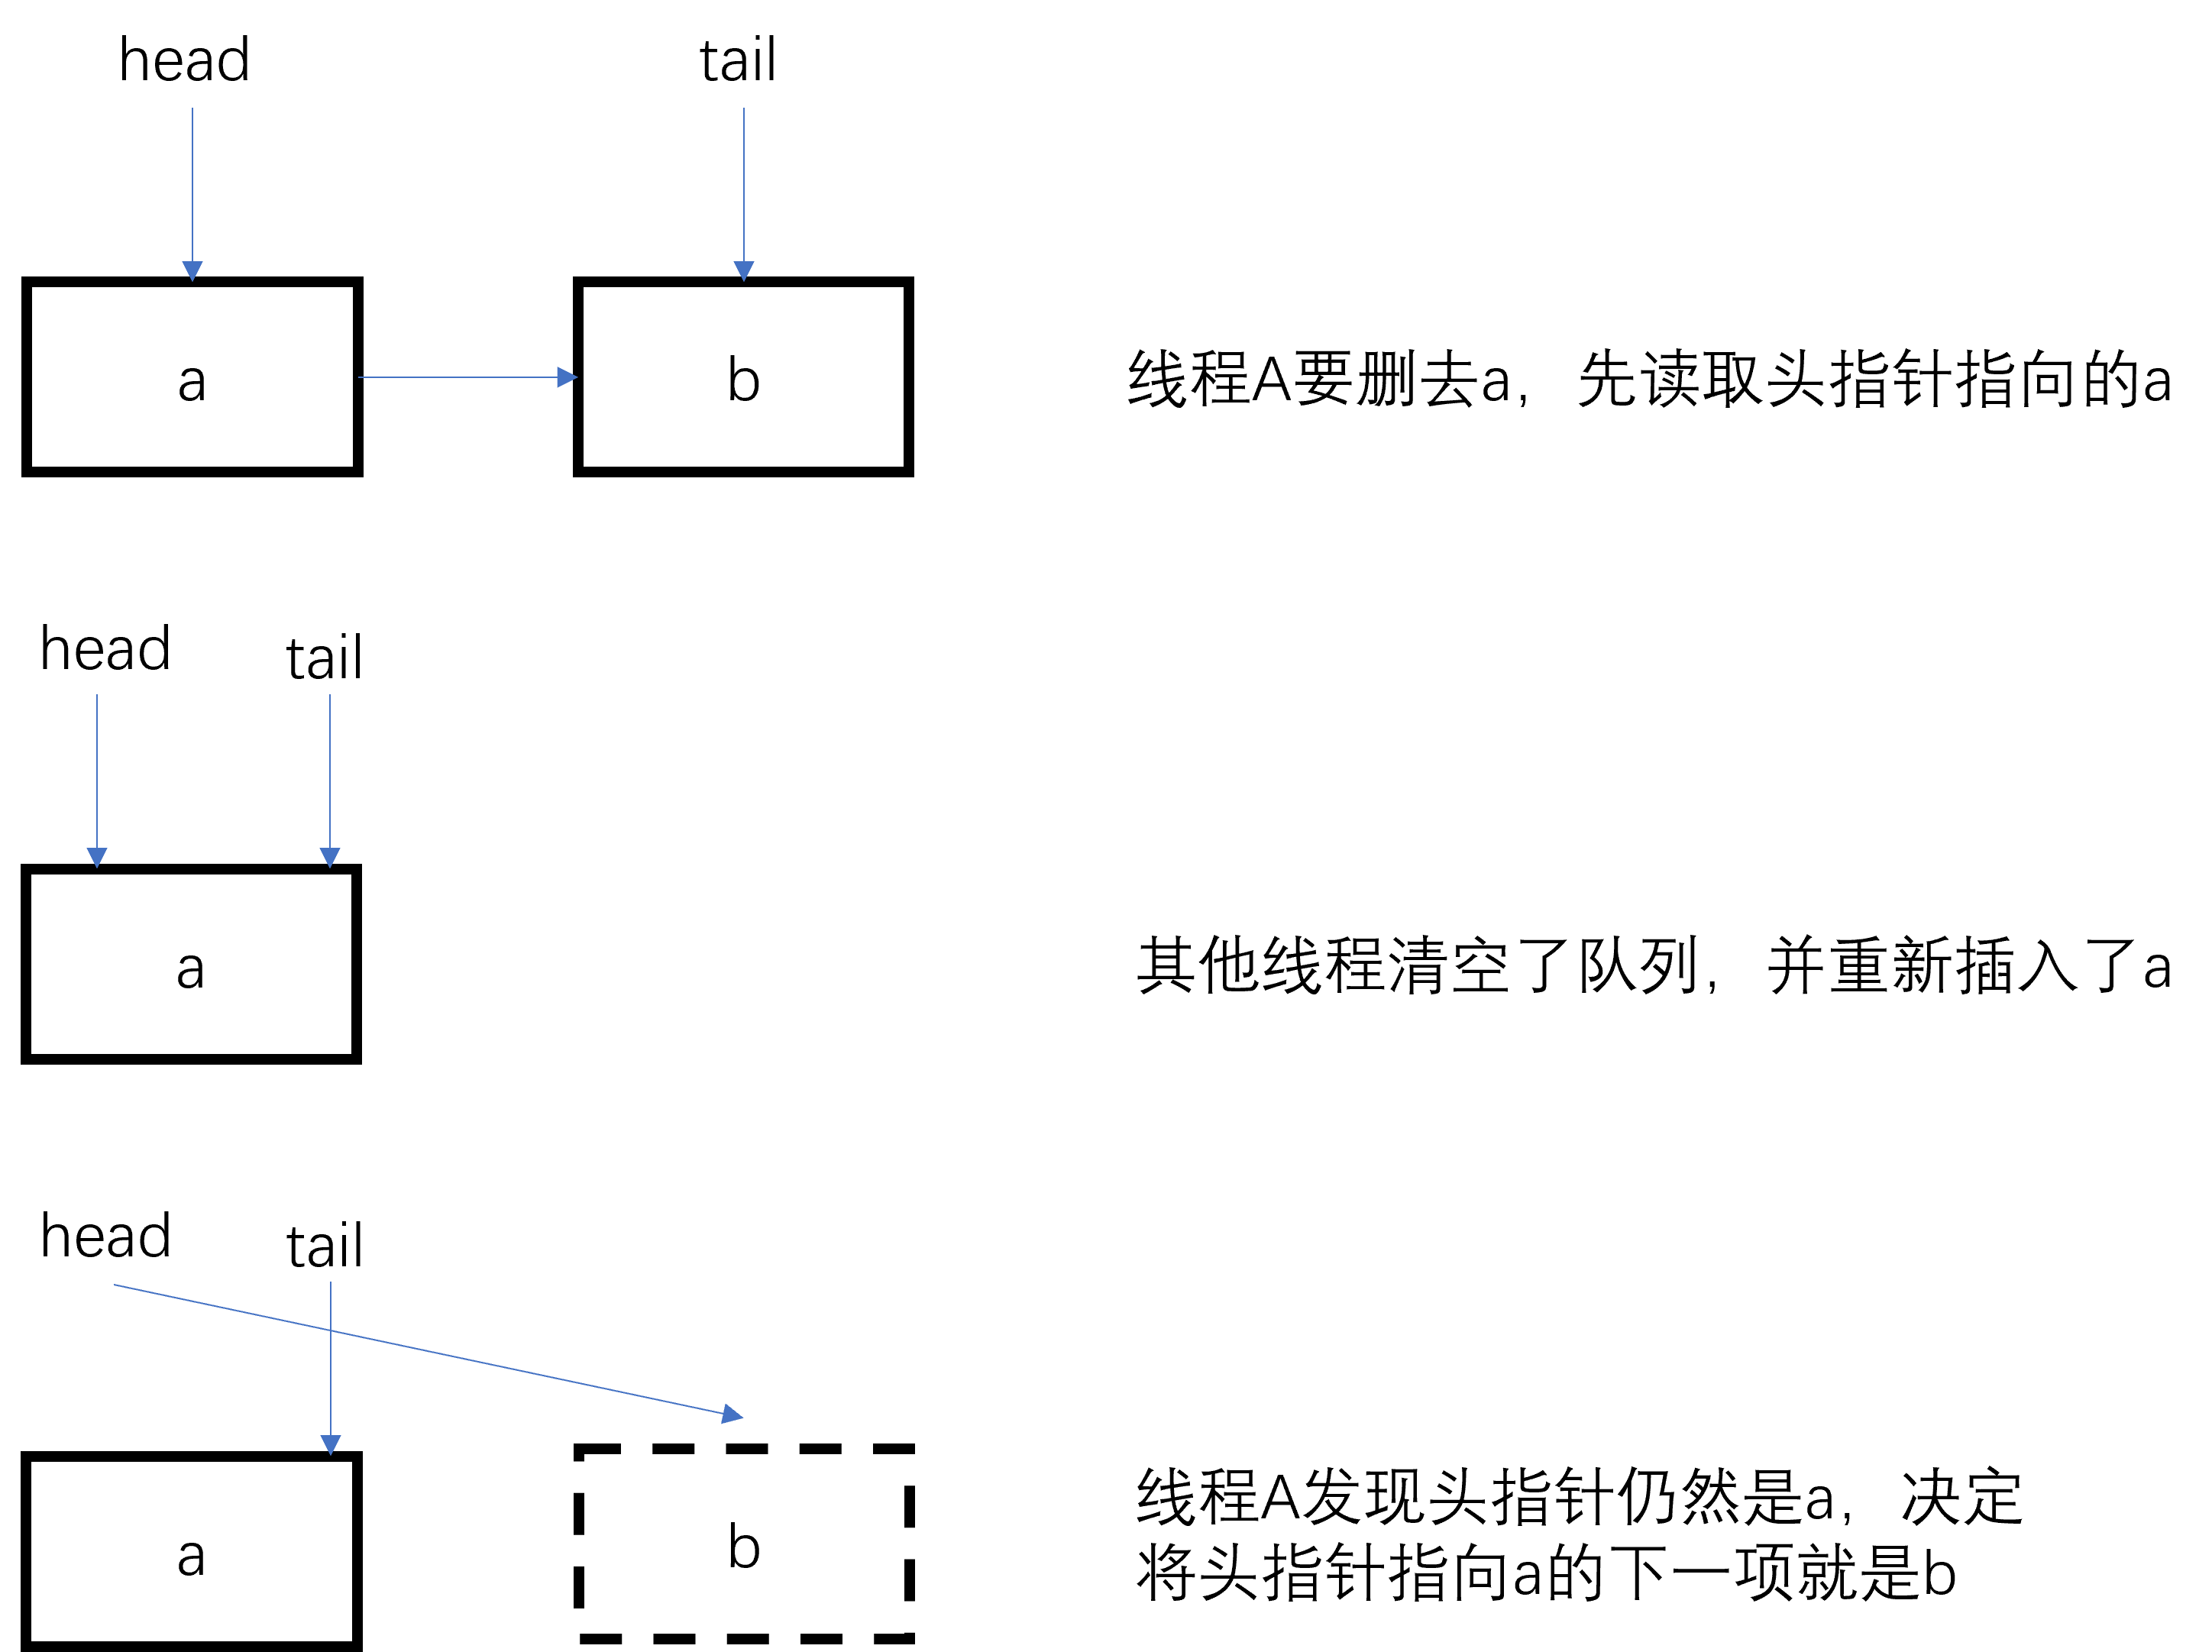
\includegraphics[width=0.8\textwidth]{图片1.png} 
    \caption{公共回收队列的ABA问题} 
    \label{fig:my_label}
\end{figure}

这个问题发生的本质原因就是,线程A根据队首元素和过去读取的元素相同,这一点判断出队首没有发生改变。这种现象就是ABA问题。上面我们提到的栈的栈顶元素不变但是栈的元素发生了改变,也是这个问题。

解决这个问题的一种直接的方法就是给每一个原子引用附上一个唯一的时间戳。每次更新的时候,时间戳加1。这样,即使两个元素相同,只要时间戳不同,那么它们就是不同的。

此外,还有一种解决方法是使用保留载入和条件存储这一对指令。保留载入是将rs1指示的存储器的内容加载到rd中,并在该存储器地址上创建一个保留。条件存储将rs2的值存储到rs1指向的存储器中。如果存在对同一内存地址的写操作破坏了对该载入的保留,那么条件存储失败并将非零值写入rd,如果成功,则将0写入rd。

利用这样的一组指令,可以检测一个值在两个时间点之间是否改变过,而不是像前面那样检测这个值在两个时间点是否刚好相等的方式来判断是否改变过。
\end{document}